\documentclass[11pt,twocolumn]{article}
\usepackage{abstract}
\usepackage{geometry}
\geometry{verbose,tmargin=3cm,bmargin=3cm,lmargin=2.5cm,rmargin=2.5cm}
\usepackage[utf8]{inputenc}
\usepackage{graphicx}
\usepackage{listings}
\lstset{
    escapeinside={(*}{*)}
}
\usepackage{appendix}
\usepackage{hyperref}
\lstset{aboveskip=24pt,belowskip=24pt}
\usepackage{mathtools}
\usepackage{amsfonts}
\usepackage{amsmath}
\lstset{language=Python}
\usepackage[english]{babel}
\usepackage[numbers]{natbib}
\usepackage{titlesec}
\usepackage{subcaption}
\usepackage{float}
\usepackage[strings]{underscore}
\usepackage{etoolbox}
\usepackage{booktabs}

\newlength{\toprulewidth}
\setlength{\toprulewidth}{0.25ex}
\patchcmd{\toprule}% <cmd>
  {\heavyrulewidth}{\toprulewidth}% <search><replace>
  {}{}% <success><failure>
  
\apptocmd{\sloppy}{\hbadness 10000\relax}{}{}

\newcommand{\floor}[1]{\left\lfloor #1 \right\rfloor}
\newcommand{\ceil}[1]{\left\lceil #1 \right\rceil}

\newcommand{\dd}[1]{\mathrm{d}#1}
\setlength{\columnsep}{0.75cm}

\newcommand*\ttvar[1]{\texttt{\expandafter\dottvar\detokenize{#1}\relax}}
\newcommand*\dottvar[1]{\ifx\relax#1\else
  \expandafter\ifx\string.#1\string.\allowbreak\else#1\fi
  \expandafter\dottvar\fi}
\usepackage{url}

% abstract styling
\renewenvironment{abstract}%
{%
  \centerline%
  {\large\bf Abstract}%
  \begin{quote}%
}
{
  \par%
  \end{quote}%
  \vskip 1ex%
}

\hypersetup{
    colorlinks=true,
    linkcolor=black,
    filecolor=black,
    citecolor=black,
    urlcolor=blue,
}


\title{\textbf{Comparison of phylogenetic reconstruction methods}}
\author{Lívia Qian\\KTH Royal Institute of Technology\\School of Electrical Engineering and Computer Science\\liviaq@kth.se}

\begin{document}

\twocolumn[
  \begin{@twocolumnfalse}
	\date{}
	\maketitle

	\begin{abstract}
The aim of this work is to briefly describe and compare the performance of five methods for phylogenetic reconstruction. Instead of trying to be a comprehensive guide summarizing the theoretical background of phylogenetics, it focuses on the main principles of creating simple phylogenetic trees and the conclusions I reached while testing these methods. My primary goal was to measure the time complexity of each algorithm besides estimating the accuracy of the generated trees. In the end, the results were compared those of the paper \textit{Confirming the Phylogeny of Mammals by Use of Large Comparative Sequence Data Sets} (Prasad et al., 2008).
    \end{abstract}
  \end{@twocolumnfalse}
]

\section{Introduction}

Phylogenetics is the study of the evolutionary history of species and groups of species. There are multiple ways to express the relationship between different groups, one of them being the construction of phylogenetic trees (or evolutionary trees) where all taxa are present as leaves. Common traits can be observed using DNA sequences or morphology, where the latter is generally more complex due to the many characteristics a certain species can have. Phylogenetic trees can be rooted and unrooted; the former is a version representing not only the similarity between different taxa but the ancestral relationships as well, while the latter only illustrates the connection between the taxonomical units.

\section{Background}

DNA is a molecule that has two polynucleotide chains forming a double helix and carries information about an organism's development and reproduction. Genomes — genetic materials that make up an organism's body — consist of both protein-coding DNA (genes) and non-coding DNA. There are four different types of nucleoids — adenine (A), guanine (G), cytosine (C) and thymine (T) — that can define the characteristics of a DNA. DNA sequencing is the process of determining the order of such nucleoids in order to gain relevant information about the molecule at hand.

DNA sequences need to be of the same length in order to be comparable with each other, therefore a proper sequence alignment is needed before one can start constructing phylogenetic trees. Sequence alignment is a way of arranging multiple DNA sequences into a matrix so that regions that show a high degree of similarity in multiple sequences are placed underneath each other. As this process can make the characters in the sequences shift, a special character (commonly a "-") is used to fill in the gaps.

There are two main categories of tree-generating algorithms \cite{DeBruyn2013}: distance-based methods are based on measuring the difference between pairs of sequences, while character-based methods use the columns of a sequence alignment directly. Examples of distance-based algorithms include neighbor joining (NJ) \cite{1987}, UPGMA \cite{sokal58}, WPGMA \cite{sokal58} and BIONJ \cite{Gascuel1997}, while the two most widely used character-based methods are the maximum parsimony (MP) and maximum likelihood (ML) methods. While all these techniques are popular, distance methods are usually recommended when computational time is an important factor; in other cases, parsimony and likelihood are preferred as they are more rigorous and have the ability to explore different combinations.

\section{Methods}

\subsection{Distance-based methods}

\subsubsection{Neighbor joining}

Neighbor joining (NJ) is a distance-based method created by Saitou and Sei in 1987 \cite{1987}. A \textit{distance matrix} is introduced as a means for storing the pairwise differences between the input sequences where the distance between two sequences is based on a predefined metric. This matrix is reduced after each step because of the clustering nature of the method.

The following steps are repeated for each iteration until there are only two nodes left:

\begin{enumerate}
\item Calculate the divergence ($r$) for every element. Divergence for element $a$ is the sum of the distances from $a$ to all the other elements.

\item Calculate the new, alternative distance matrix using the following formula:
\begin{align}
d_{new}(i, j) = d(i, j) - \frac{r(i) + r(j)}{N - 2}
\end{align}
where $N$ is the number of elements in the current iteration.

\item Take the smallest value in the new distance matrix and the elements belonging to it (let them be denoted by $a$ and $b$). Let $p$ be a new node that represents the common parent of $a$ and $b$. The length of the new branches can be calculated as
\begin{align}
\delta(a, p) = \frac{d(a, b)}{2} + \frac{r(a) - r(b)}{2 (N - 2)} \\
\delta(b, p) = d(a, b) - \delta(a, p)
\end{align}

\item The rows and columns belonging to $p$ need to be added to the original distance matrix, while the ones belonging to $a$ and $b$ need to be deleted. After this, the difference between $p$ and the remaining nodes need to be calculated. Let's take an arbitrary element $c$ as an example:
\begin{align}
d(c, p) = \frac{d(a, c) + d(b, c) - d(a, b)}{2}
\end{align}
Branches $(a, p)$ and $(b, p)$ are now part of the tree that is being built.

\end{enumerate}

After this, the remaining two elements can be joined by taking the ancestral node created in the last iteration, i.e., one of these two nodes, and making the other one its child with their distance that was specified in the last iteration as the branch length.

Although it was originally intended for unrooted trees, NJ can easily be extended to rooted trees. This is one of the simplest and fastest methods in phylogeny, but it may not produce accurate results due to its simplicity.

\subsubsection{WPGMA}

Originally attributed to Sokal and Michener \cite{sokal58}, WPGMA (weighted pair group method with arithmetic mean) is a hierarchical clustering method that uses a distance matrix in a similar fashion as the neighbor joining method. Each step consists of the following and is repeated until there is only one node left:

\begin{enumerate}
\item Find the smallest element in the distance matrix. Suppose that it is $d(a, b)$, therefore it belongs to elements $a$ and $b$ (both of them can be clusters). Create a parent node called $p$.

\item Calculate branch lengths $\delta(a, p)$ and $\delta(b, p)$. If both $a$ and $b$ are leaves, these lengths are simply
\begin{align}
\delta(a, p) = \delta(b, p) = \frac{d(a, b)}{2}
\end{align}
If $a$ or $b$ is a cluster, the height of the subtree that belongs to them needs to be subtracted from $\frac{d(a, b)}{2}$ to get the  corresponding branch length. Suppose that $a$ is a cluster and that $c$ is a leaf of the subtree belonging to it. In this case,
\begin{align}
\delta(c, p) = \frac{d(a, b)}{2}
\end{align}
\begin{align}
\begin{split}
\delta(a, p) = \delta(c, p) - \delta(c, a) = \\
= \frac{d(a, b)}{2} - \delta(c, a)
\end{split}
\end{align}

In the case where $a$ is a leaf, $c$ could be represented by $a$ itself and $\delta(c, a)$ would be zero, therefore this is a generalized formula that can be used in any situation.

\item After cluster $p = (a, b)$ is created, it should be integrated into the distance matrix as a new element; for this purpose, a new column and a new row should be created and the columns and rows belonging to $a$ and $b$ may be deleted. The distance between $p$ and any arbitrary element $q$ can be calculated as
\begin{align}
\begin{split}
d(p, q) = d((a, b), q) = \\
= \frac{d(a, q) + d(b, q)}{2}
\end{split}
\end{align}
This step is not needed in the last iteration.

\end{enumerate}

\subsubsection{UPGMA}

Also created by Sokal and Michener \cite{sokal58}, UPGMA (unweighted pair group method with arithmetic mean) is highly similar to WPGMA. The only difference lies in that it keeps track of the number of elements in each cluster, making the resulting calculations unweighted. In Step 3, UPGMA uses cluster weights, resulting in the following distance matrix update rule:
\begin{align}
d((a, b), q) = \frac{d(a, q) \cdot m + d(b, q) \cdot n}{m + n}
\label{eq:upgma}
\end{align}
where $a$ consists of $m$ and $b$ consists of $n$ elements. This is called \textit{proportional averaging}.

There are situations in which it is not recommended to use UPGMA, e.g., when the three-point criterion is not fulfilled. This criterion demands that for any three elements $d(a, c) \le max(d(a, b), d(b, c))$, i.e., that the two greatest distances be equal. This is needed because UPGMA assumes a constant rate of evolution across lineages, therefore none of the leaves can be further away from the root than the others.

\subsection{Character-based methods}
\subsubsection{Maximum parsimony}

Maximum parsimony (MP) is an umbrella term for all the methods that are based on the principle that a model is better than another if it implies fewer evolutionary events. The number of evolutionary events is represented by a cost called the \textit{parsimonious score}. There are two major categories: \textit{exact} methods are the ones that consider the score of all possible trees, thus giving a global minimum, and \textit{heuristic} methods are those that use some kind of technique to find a significant subset of all the trees and produces a somewhat sub-optimal result. As exact methods are often computationally infeasible, it is recommended to use a heuristic method and let it run for a sufficient amount of time.

Fitch's algorithm \cite{Fitch1971} can be used to calculate the score of an input tree  \cite{Ortiz2016}\cite{Stoye2009}: the first-pass of the algorithm starts from the leaves and goes up to the root to determine the parsimonious score and possible sets of bases at each internal node, while the second-pass goes from top to bottom and helps in determining a hypothetical tree. In each step of the first phase, the algorithm takes a look at the bases belonging to the children nodes (which consist of one element in the case of the leaves), and then, assigns their intersection to the parent node if they have bases in common. If they do not have any bases in common, the parent node gets the union of the children's sets and the parsimonious score is increased by 1. This algorithm is repeated for each site — that is, position in the sequences — in all input sequences and the score is summed up in the end.

There is a number of heuristic methods that can help in exploring new trees, for example nearest neighbor interchange (NNI), subtree pruning and regrafting (SPR), or tree bisection and reconnection (TBR) \cite{felsenstein2004}. NNI is the simplest one but is used for unrooted binary trees; the current tree may produce two new trees if all four branches connecting to one of its internal branches are swapped in every possible combination. In SPR, a certain subtree is removed from the current tree and gets reinserted elsewhere. TBR does the same as SPR, but instead of reinserting the subtree in the form it was in originally, it tries every possible way of connecting the two subtrees; similarly to NNI, it works for unrooted trees only. These methods are stochastic, but they should be able to approximate the original distribution of trees given that they have enough time to run.

Branch and bound, an exact method that filters out a certain number of trees, may reduce the running time of the exhaustive search significantly. This is a method that considers all possible trees but makes use of the fact that adding a new edge to a tree increases its parsimonious score, thus avoids going for trees that are bigger than the current one in each step.

\subsubsection{Maximum likelihood}

Maximum likelihood (ML), like in many cases where probabilistic methods are used, makes use of the basics of Bayesian statistics and examines the probability of a certain sequence given a model; the higher the probability the better the model. In some cases, the relationship between successive sites — characters — is the driving factor in determining the best model, e.g., in Hidden Markov models, where transition matrices are used for storing such information. It may have a high algorithmic complexity as evaluating one sequence in itself can be computationally intensive, let alone multiple sequences. Additionally, there are Bayesian methods (e.g., Markov chain Monte Carlo) that build upon ML; the major difference between these two groups of tree-building algorithms is that Bayesian methods take prior knowledge into account.

\subsection{Self-growing tree algorithm}

Self-growing tree algorithm (or self-organizing tree algorithm) is based on a paper published in 1997 by Dopazo and Carazo \cite{Dopazo1997} and is a combination of the Kohonen self-organizing map \cite{58325} and the growing cell structures algorithm of Fritzke \cite{Fritzke1994}. This is an unsupervised learning network that first initializes a tree consisting of a small number of nodes (the paper mentions two sister nodes) and then alternates between growing the tree and adapting it to the input sequences until it is fully grown and every taxonomic unit is assigned a proper place. The strictest exit condition guarantees that every input sequence is associated to a unique cell.

First, the input sequences are converted to one-hot encoded values. Secondly, the tree's initial node(s) and the corresponding weight matrices that the encoded input sequences will ultimately be compared to need to be created; in order to distinguish inner nodes from leaves, the authors of the paper mention that it would be best to call them \textit{nodes} and \textit{cells}, respectively. In each step, nodes are considered "closed", meaning that they cannot be assigned sequences after they transition from being a cell to a node. After the first few cells are initialized with numbers ranging from 0 to 1, the alternating phases begin to take place. The first phase is called adaptation, which is basically what characterizes Kohonen's self-organizing maps: the input points are compared to all available cells and those that are closest to each of the inputs are updated, along with their neighborhood (in the paper, finding the winning cell and updating its neighborhood is referred to as a \textit{presentation}). After running this for a number of epochs, the inputs are mapped to appropriate positions in the output space, namely, the cells that they are the closest to according to a predefined metric. This distance metric is defined as
\begin{align}
d_{S_j C_j} = \frac{\sum_{r = 1}^A S_j(r, l) \cdot C_i(r, l)}{L}
\end{align}
where $S_k$ is sequence $k$, $C_i$ is cell $i$, $A$ is the number of characters in the alphabet (in our case, four) and $L$ is the length of the sequences.

The concept of neighborhood is not as intuitive as when the output space is a 1D or 2D space; in the case where the winning cell's sister is a cell, the winning cell, the sister cell and their common ancestor (mother cell) all get updated — it should be noted that all three of them are assigned different update rates. However, if the sister is actually a subbranch of the tree and consists of multiple nodes and cells, only the winning cell is updated.

The second phase is the growing of the tree. As it is mentioned in the paper \cite{Dopazo1997}, "the growing of the network takes place in the cell having higher resources. This cell gives rise to two new descendant cells [...] and transforms itself into a node. At this moment, its upper node becomes a grandmother node, and thereafter, it does not receive any more updating. The two new cells are, in principle, identical to the node which generated them".

The tree stops growing when the resource value of the cell with the highest value is smaller than a predefined threshold — this threshold should be zero if the goal is to map each sequence to a unique cell, or rather, a sufficiently small number in order to avoid inaccuracies in numerical calculations. The concept of resource value is related to the distance between cells and input points, and is defined as
\begin{align}
R_i = \frac{\sum_{k = 1}^K d_{S_k C_i}}{K}
\end{align}
where $R$ is the resource value belonging to cell $i$, $S_k$ is sequence $k$, $C_i$ is cell $i$ and the summation is done over the $K$ sequences associated to cell $i$.

The criteria used for monitoring the convergence of the network relies on the definition of the total error, $\epsilon$, "defined as the summation of the distances of each sequence to the corresponding winning cell after an epoch" \cite{Dopazo1997}. This helps in setting an exit condition for the adaptation process — e.g., the process can be ended when the relative increase of the error falls below a small threshold. The relative increase in error is
\begin{align}
\Big|\frac{\epsilon_t - \epsilon_{t-1}}{\epsilon_{t-1}}\Big| < E
\end{align}

What is also interesting is that there is an extended update rule that is based on Kohonen's original formula:
\begin{align}
C_i(\tau + 1) = C_i(\tau) + \eta_{t, \tau, i} \cdot [S_j - C_i(\tau)]
\end{align}
and $\eta_{t, \tau, i}$ is defined as a factor dependent on the number of cycles among others:
\begin{align}
\eta_{t, \tau, i} = \alpha_i \cdot \frac{1 - t}{M_t} \cdot (1 - b\tau)
\end{align}
where $\alpha_i$ is a coefficient dependent on the role of the current cell, $t$ is the total number of presentations, $M_t$ is the maximum number of presentations allowed ($\mu \times A \times L$) and $b$ is the
slope for the reduction of the interaction as the number of presentations, $\tau$, increases within a cycle.

\section{Data}

The first dataset I used is a protein-coding sequence alignment \cite{dataset} consisting of 44 sequences of different vertebrate taxa. The input is first processed by Biopython's sequence alignment class before being passed to any of the algorithms implemented. Since this dataset was evaluated in a 2008 paper by Prasad et al. \cite{Prasad2008}, I decided to compare my results with those published in this work. From now on, I will refer to this dataset as the \textit{coding dataset}. The other dataset I ran my experiments on uses non-coding DNA sequences but is identical to the coding dataset in every other aspect \cite{dataset}; I will refer to this as the \textit{non-coding dataset}. Both datasets were stored in FASTA format which is a text-based format for describing nucleotide or protein sequences. For comparison, the coding dataset contains 16016 lines and 978129 characters in total (including FASTA description lines), while the non-coding datasets consists of 97196 lines and 5924564 characters. The sequence alignments created from these datasets contain sequences of length 21510 and 132423, respectively.

%For the experiments I conducted, I assumed that the relationship between the speed of my algorithms holds for different datasets.

\section{Implementation}

I implemented the algorithms mentioned in the previous section using Python 3 with NumPy and Pandas. For some of these, I used Biopython v1.77 as a reference or benchmark (see Appendix \ref{sec:functionality_testing}). Since some of the data structures needed were not feasible to implement within the scope of the project, I decided to use Biopython's corresponding classes to facilitate the work; these are \ttvar{Bio.SeqIO}, \ttvar{Bio.Align.MultipleSeqAlignment}, \ttvar{Bio.Alphabet} and \ttvar{Bio.Phylo.BaseTree}. They were needed to read in data, create sequence alignments in the format needed, fill in the gaps in the sequence alignments and create the trees in a form that can be visualized easily, respectively.

I decided to use rooted trees because they are generally more accurate and easily comparable. Biopython's \ttvar{BaseTree} can easily be visualized with \ttvar{Bio.Phylo.draw}, a function that supports features like custom branch lengths and node labels.

The methods I implemented are neighbor joining, UPGMA, WPGMA, maximum parsimony and SOTA. In the case of MP, I implemented an exact algorithm that uses exhaustive search to find all the trees and a heuristic algorithm that uses SPR (I will refer to them as \textit{exact} and \textit{heuristic} method, respectively). The exact method has an additional option for branch and bound, which can increase its speed dramatically. SOTA contains a few hyper-parameters that can be tuned before extensive testing. I found that the following parameters provided a relatively fast convergence: $\alpha_w = 0.5$ (current cell's update rate), $\alpha_m = 0.02$ (mother cell's update rate), $\alpha_s = 0.01$ (sister cell's update rate), $b = 0$ (slope), $\eta = 0.5$ (learning rate).

\section{Experiments}

First of all, I tested which version or parameters of a certain algorithm would be the best for the main experiments. The three distance-based methods do not need any fine-tuning, therefore there were only two methods that needed optimization. After this, I compared the five main algorithms with respect to running time and performance.

\subsection{Maximum parsimony — versions}

\begin{figure*}
	\centering
	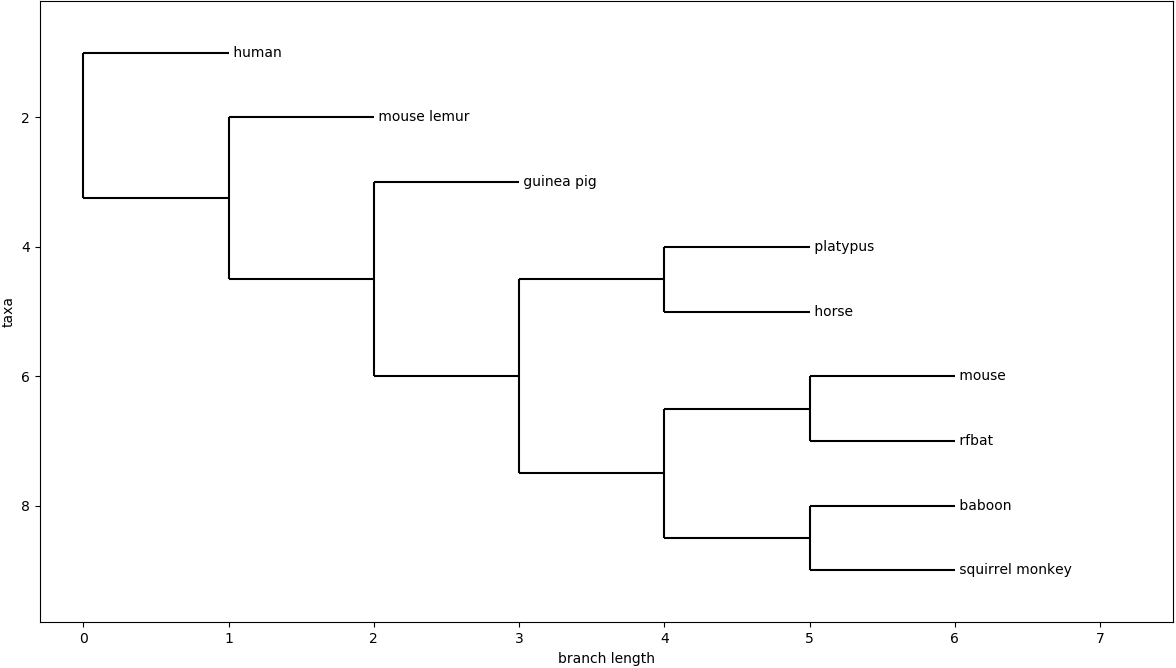
\includegraphics[width=0.85\linewidth]{img/mp_9_taxa_heuristic.png}
	\caption{The result of running the heuristic MP method on 8 elements of the coding dataset. The tree shown in this figure is the one with the highest score after 50 iterations.}
	\label{fig:mp_8_taxa_heuristic}
\end{figure*}

While the exact method does not rely on any parameters (branch and bound produces the same result as the full version), heuristic MP with SPR needs the maximum number of iterations — that is, the number of trees to test — as input. The heuristic version needs to run for a relatively long time to find a sufficiently good result; because of its stochastic nature, the use of optimization methods may boost both its performance and speed. For the main experiments, I decided to test the exact method instead of the heuristic one as it is able to produce optimal results under all circumstances.

Figure \ref{fig:mp_8_taxa_heuristic} shows a tree resulting from a 50-iteration heuristic MP that has run on 9 randomly selected species; although the algorithm managed to find some smaller clusters (\textit{baboon} and \textit{squirrel monkey}, \textit{mouse} and \textit{bat}), the results are still far from optimal.


\subsection{Hyper-parameters of SOTA}

There are multiple parameters that can define the self-organizing tree algorithm, including the three $\alpha$ values (update rates of the current cell, sister cell and mother cell), the slope ($b$) and the learning rate ($\eta$). In Table \ref{table:sota_parameters}, I listed the configurations I tried on a dataset consisting of 5 taxa; for all cases, the condition $\alpha_w > \alpha_m > \alpha_s$ mentioned in the original paper \cite{Dopazo1997} was satisfied. Out of the configurations that managed to converge within 50 iterations, I chose the first one because it seemed to provide a good balance between running time and parameter values, assuming that a smaller (but not too small) learning rate is preferable over values like 1 and 2. One can perform a grid search to find the most optimal configuration, but defining what it means is not trivial, as not only the speed but the resulting tree also counts. Moreover, the concept of good parameters is highly dependent on the dataset and the task at hand.

\begin{table}[H]
	\caption{Different combinations of the SOTA parameters, the corresponding speed averaged over two runs and the answer to whether the algorithm converged after 50 iterations for all runs. Convergence means that all species have been assigned a leaf in the resulting tree.}
	\centering
	\begin{tabular}{lllllll}
		\toprule
		$\alpha_w$ & $\alpha_m$ & $\alpha_s$ & $b$ & $\eta$ & Time (s) & Co. \\
		\midrule
		0.5 & 0.02 & 0.01 & 0 & 0.5 & 89.0312 & Y \\
		0.5 & 0.02 & 0.01 & 0 & 1 & 44.1286 & Y \\
		0.5 & 0.025 & 0.02 & 0 & 0.5 & 81.517 & Y \\
		0.05 & 0.02 & 0.01 & 0 & 0.5 & 433.4081 & N \\
		0.05 & 0.02 & 0.01 & 0 & 1 & 225.1199 & N \\
		0.05 & 0.02 & 0.01 & 0 & 2 & 148.2399 & Y \\
		\bottomrule
	\end{tabular}
	\label{table:sota_parameters}
\end{table}

\section{Results}

\subsection{Comparison of running time}

All the experiments were run on CPU (Intel Core i7-8650U, 1.9 GHz); none of the algorithms were optimized for GPU which made testing hard to a certain extent. Some methods were computationally intensive (e.g, maximum parsimony with 9 species and SOTA with 44 species), therefore I will include the result of only one test run in these cases. Most of the results in this section were created using the coding dataset.

\begin{table}[H]
  \caption{Running time of the distance-based methods on the coding dataset. 44 taxa are used. The numbers are based on three test runs.}
  \centering
  \begin{tabular}{lll}
    \toprule
    Method & Mean (seconds) & Std. \\
    \midrule
    NJ & 3.3105 & 0.3885 \\
    UPGMA & 0.6767 & 0.0446 \\
    WPGMA & 0.5359 & 0.0526 \\	
    \bottomrule
  \end{tabular}
\label{table:distance}
\end{table}

\begin{table}[H]
  \caption{Running time of the exact maximum parsimony method on the coding dataset. Uses branch and bound. Based on three test runs (except for the case with 9 taxa).}
  \centering
  \begin{tabular}{lll}
    \toprule
    Nr. of taxa & Mean (seconds) & Std. \\
    \midrule
    6 & 43.9988 & 2.7520 \\
    7 & 916.6252 & 661.2072 \\
    8 & 8613.8869 & 5145.0788 \\
    9 & 228420.7188 & - \\
    \bottomrule
  \end{tabular}
\label{table:mp}
\end{table}

\begin{table}[H]
  \caption{Running time of the self-growing tree algorithm on the coding dataset. Based on three test runs (except for the case with 44 taxa).}
  \centering
  \begin{tabular}{lll}
    \toprule
    Nr. of taxa & Mean (seconds) & Std. \\
    \midrule
    4 & 53.8339 & 4.49524 \\
    5 & 93.3756 & 3.4764 \\
    6 & 117.2846 & 0.5958 \\
    7 & 182.7518 & 8.5831 \\
    15 & 2399.81665 & 464.18335 \\
    44 & 36669.3622 & - \\
    \bottomrule
  \end{tabular}
\label{table:sota}
\end{table}

It can be seen that the three distance-based methods are immensely fast, especially since they do not entail convoluted tree-manipulation steps. SOTA runs in a sensible amount of time, and it may be reasonable to think that it can provide a better solution than NJ, UPGMA and WPGMA at the same time as being able to keep its running time under control for a dataset of this size.

What I noticed during the creation of the tree shown in Figure \ref{fig:sota_noncoding} is that it took much more time than the one shown in Figure \ref{fig:sota} (309065.822 seconds, to be precise). It can be assumed that the running time of the exact MP would be much higher for not only the coding dataset but also for the non-coding dataset. In order to justify this, I compared these two algorithm's performance on the non-coding dataset with smaller numbers of taxa. The results are shown in Tables \ref{table:mp_noncoding} and \ref{table:sota_noncoding}.

\begin{table}[H]
	\caption{Running time of the exact maximum parsimony method on the non-coding dataset. Based on two test runs.}
	\centering
	\begin{tabular}{lll}
		\toprule
		Nr. of taxa & Mean (seconds) & Std. \\
		\midrule
		6 & 278.8148 & 4.8364 \\
		8 & 18598.8609 & 1880.5376 \\
		\bottomrule
	\end{tabular}
\label{table:mp_noncoding}
\end{table}

\begin{table}[H]
	\caption{Running time of the self-growing tree algorithm on the non-coding dataset. Based on two test runs.}
	\centering
	\begin{tabular}{lll}
		\toprule
		Nr. of taxa & Mean (seconds) & Std. \\
		\midrule
		6 & 825.4406 & 15.2346 \\
		8 & 1683.4831 & 2.2107 \\
		\bottomrule
	\end{tabular}
\label{table:sota_noncoding}
\end{table}

\subsection{Comparison of accuracy}

\subsubsection{Coding dataset}

\begin{figure*}
    \centering
    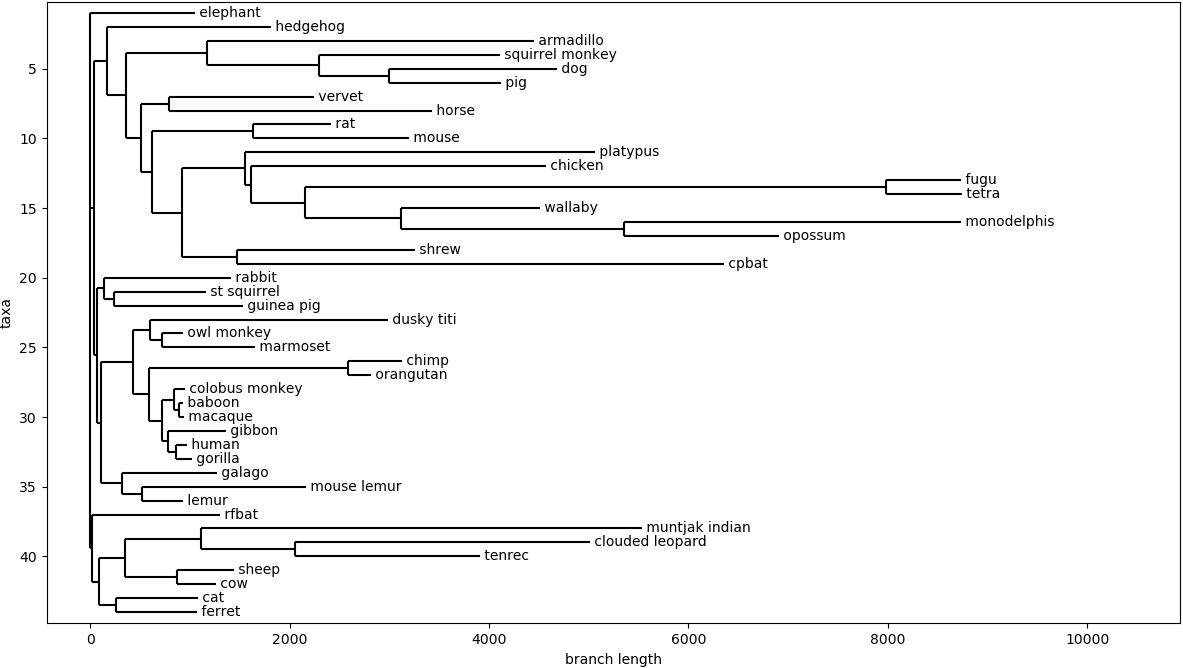
\includegraphics[width=\linewidth]{img/nj.png}
    \caption{The result of running neighbor joining on the coding dataset.}
    \label{fig:nj}
\end{figure*}

\begin{figure*}
    \centering
    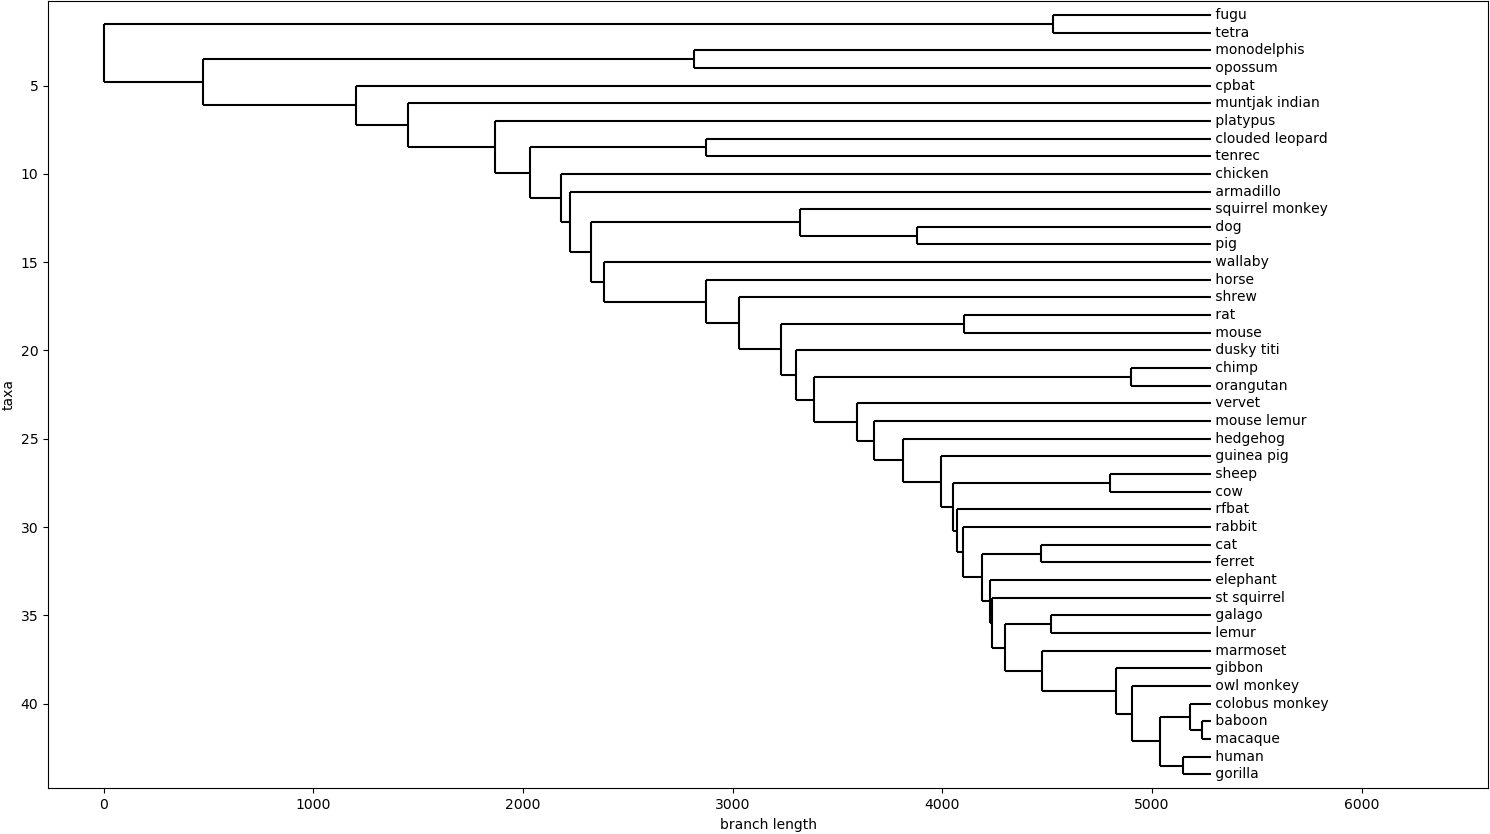
\includegraphics[width=\linewidth]{img/upgma.png}
    \caption{The result of running UPGMA on the coding dataset.}
    \label{fig:upgma}
\end{figure*}

\begin{figure*}
    \centering
    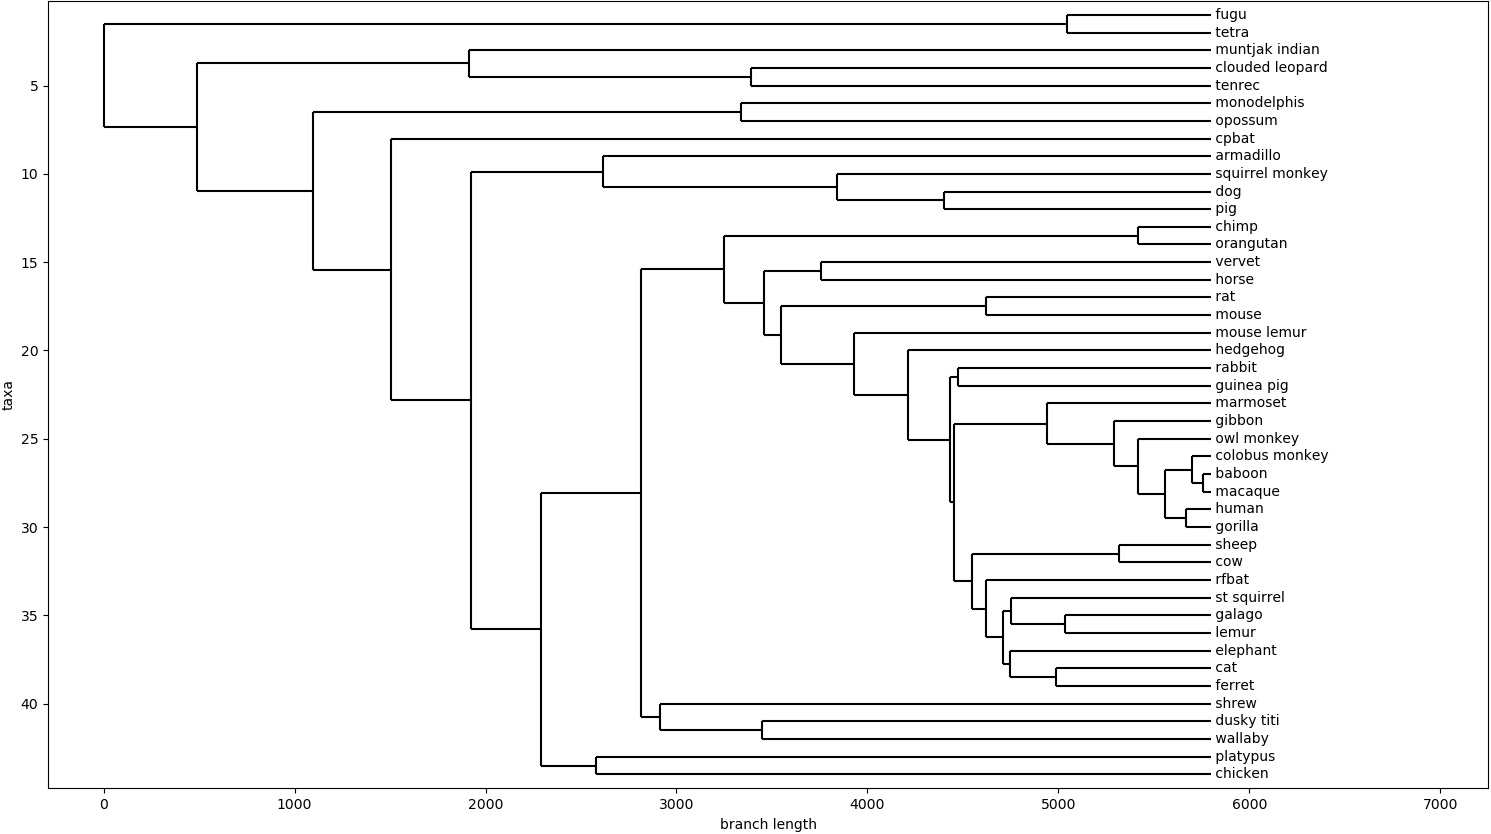
\includegraphics[width=\linewidth]{img/wpgma.png}
    \caption{The result of running WPGMA run the coding dataset.}
    \label{fig:wpgma}
\end{figure*}

\begin{figure*}
    \centering
    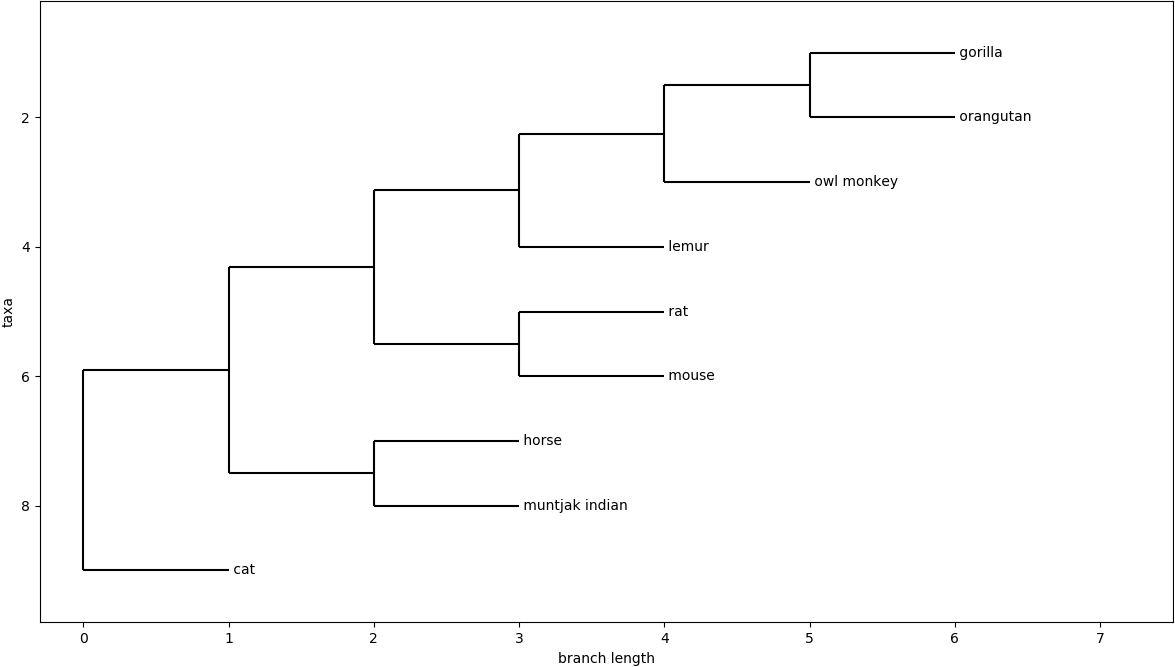
\includegraphics[width=\linewidth]{img/mp_9_taxa.png}
    \caption{The result of running the exact MP method with branch and bound on 9 elements of the coding dataset. Branch lengths have been adjusted to the parsimonious scores of the nodes.}
    \label{fig:mp}
\end{figure*}

\begin{figure*}
    \centering
    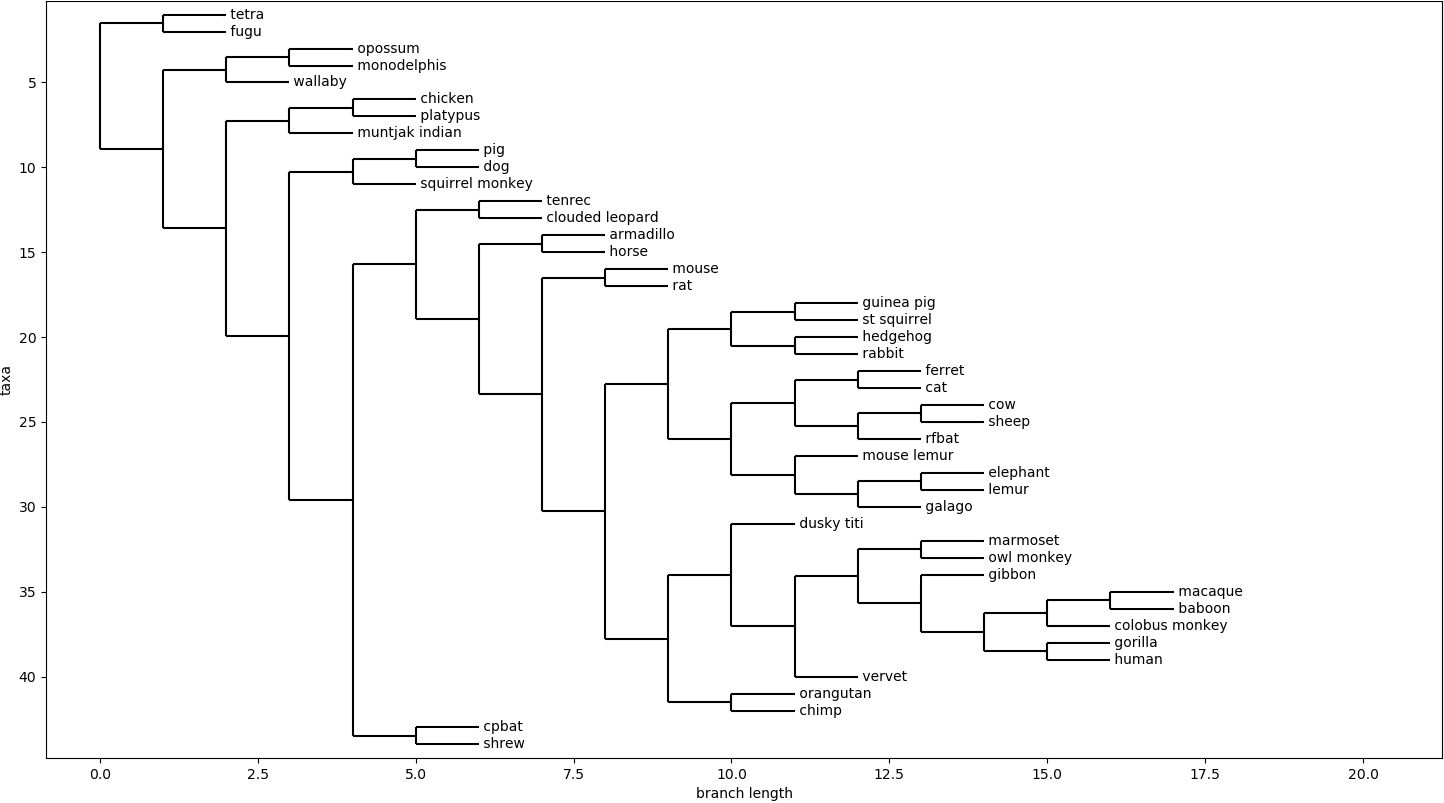
\includegraphics[width=\linewidth]{img/sota.png}
    \caption{The result of running SOTA on the coding dataset.}
    \label{fig:sota}
\end{figure*}

I tested the algorithms on the coding dataset first. Regarding the tree created with neighbor joining (Figure \ref{fig:nj}), we can see that \textit{cats} and \textit{ferrets} are closely related (Carnivora, Laurasiatheria, Boreoeutheria), but they are further away from \textit{dogs} and \textit{pigs} which should be closely related to them according to the point of reference \cite{Prasad2008}. \textit{Sheep} and \textit{cows} are related (Cetartiodactyla), as well as species that are close to \textit{humans} (baboon, orangutan, chimp, gorilla, colobus monkey, macaque, gibbon). Neighbor joining managed to position other primates in the same cluster as well. The algorithm did well by placing some rodents in the vicinity of primates; it, however, put \textit{rats} and \textit{mice} into a different high-level category as humans. Other discrepancies include putting mostly dissimilar species like \textit{muntjak} and \textit{clouded leopard} next to each other but it can be said that it performed fairly well, especially since it is the most basic method.

When it comes to UPGMA (Figure \ref{fig:upgma}), cats and ferrets are still far from dogs and pigs but munjaks and leopards moved further from each other. Besides this, it performed a little worse than neighbor joining; \textit{chimps} and \textit{orangutans} have moved away from other primates, and other high-level categories remained mixed or obscure. Closely tied species still go together — \textit{tetraodon-fugu}, \textit{sheep-cow}, \textit{baboon-macaque}, \textit{rat-mouse}, \textit{human-gorilla} —, but other highly similar species — \textit{muntjak-cow}, \textit{horseshoe bat and short-tailed bat}, \textit{mouse lemur and right-tailed lemur}, \textit{owl money and squirrel monkey}, \textit{short-tailed opossum (monodelphis) and North American opossum (opossum)} — are separated from each other.

In the case of WPGMA (Figure \ref{fig:wpgma}), only the mid-level clusters seem to have moved around compared to the structure of the tree produced by UPGMA. Most of the statements that apply to UPGMA are true of WPGMA as well. Slight improvements can be seen in certain relationships, e.g. \textit{platypuses} and \textit{chickens} got paired up and \textit{guinea pigs} got closer to \textit{rats} and \textit{mice}; these changes, however, are not sufficient to claim that there is a significant difference in UPGMA and WPGMA.

As mentioned before, time is an important factor when using maximum parsimony. The maximum number of taxa I ran the exact method on was 9, therefore only a subtree of the result is shown in Figure \ref{fig:mp}. The exact method has the capacity to evaluate every possible combination of branches, therefore the solution it provides is optimal. It can be said that the resulting tree bears a high degree of resemblance to Figure 1 in Prasad's paper \cite{Prasad2008}.

Finally, SOTA (Figure \ref{fig:sota}) created a tree that has guessed the major clusters right, but there are minor disparities in less obvious cases: \textit{muntjak} is grouped with \textit{chicken} and \textit{platypus}, \textit{squirrel monkey} is with \textit{pig} and \textit{dog} and \textit{tenrec} belongs to the same branch as \textit{clouded leopard}. It was generally good at identifying the similarities between different primate and rodent species, but there is still room for improvement, for example, \textit{shrew} and one of the \textit{bat} species have diverged from the other species of \textit{Laurasiatheria}.

\subsubsection{Non-coding dataset}

\begin{figure*}
    \centering
    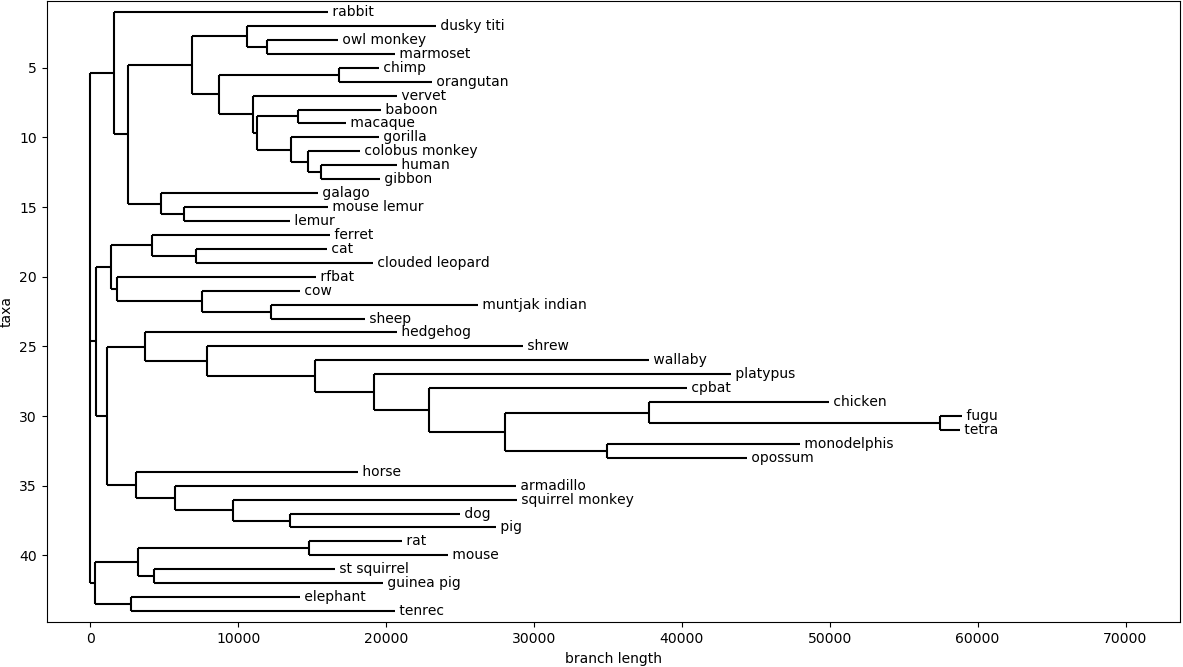
\includegraphics[width=\linewidth]{img/nj_noncoding.png}
    \caption{The result of running neighbor joining on the non-coding dataset.}
    \label{fig:nj_noncoding}
\end{figure*}

\begin{figure*}
    \centering
    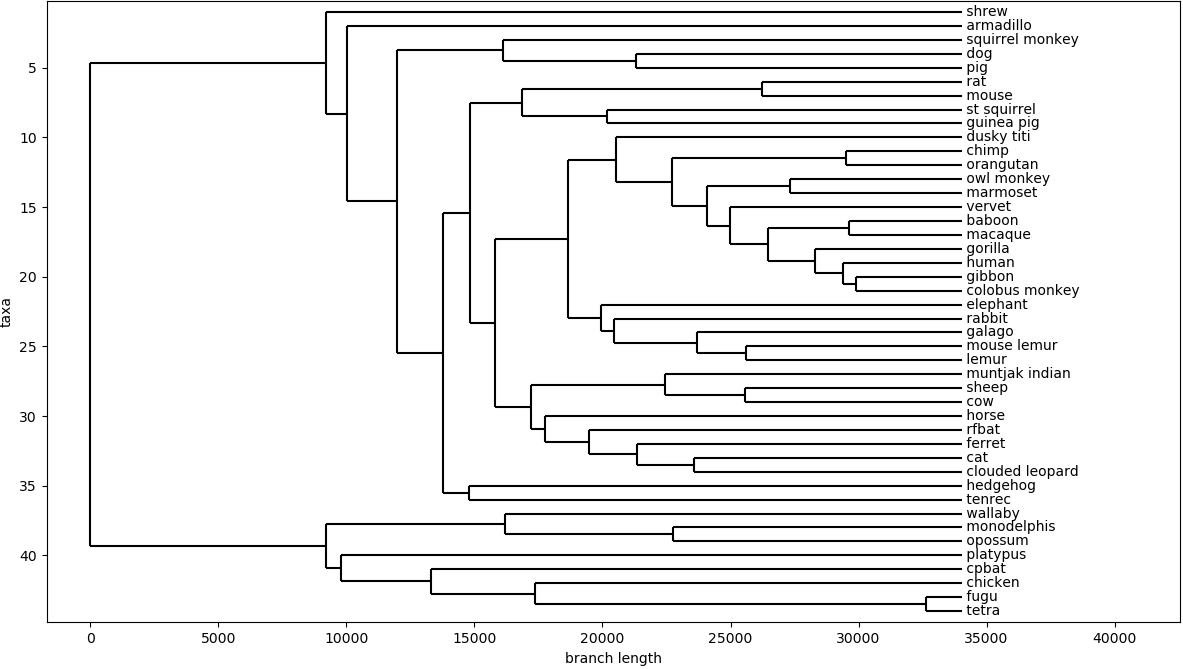
\includegraphics[width=\linewidth]{img/upgma_noncoding.png}
    \caption{The result of running UPGMA on the non-coding dataset.}
    \label{fig:upgma_noncoding}
\end{figure*}

\begin{figure*}
    \centering
    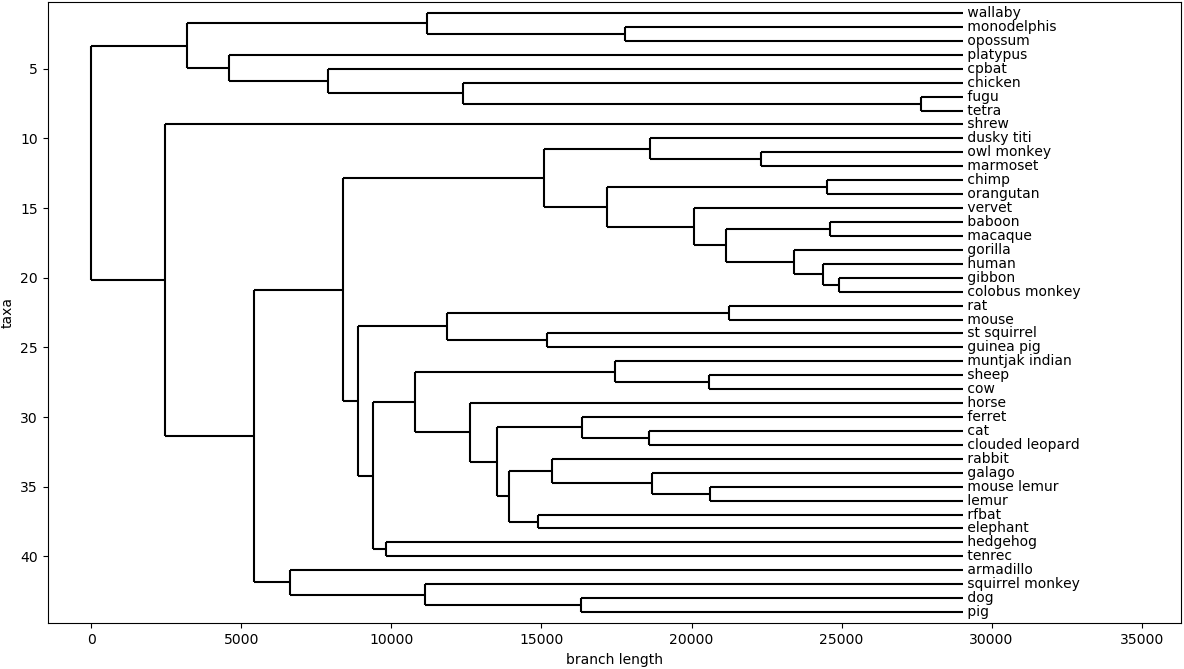
\includegraphics[width=\linewidth]{img/wpgma_noncoding.png}
    \caption{The result of running WPGMA on the non-coding dataset.}
    \label{fig:wpgma_noncoding}
\end{figure*}

\begin{figure*}
    \centering
    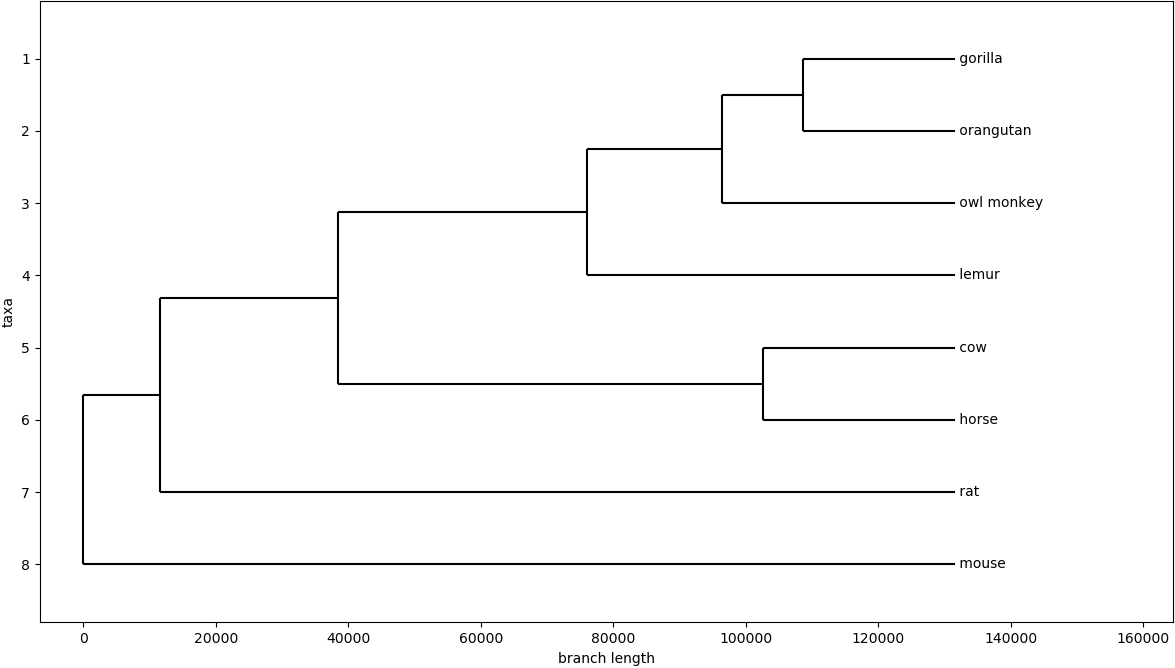
\includegraphics[width=\linewidth]{img/mp_8_taxa_noncoding_1.png}
    \caption{The result of running the exact MP method with branch and bound on 8 elements of the non-coding dataset. Branch lengths have been adjusted to the parsimonious scores of the nodes.}
    \label{fig:mp_noncoding_1}
\end{figure*}

\begin{figure*}
    \centering
    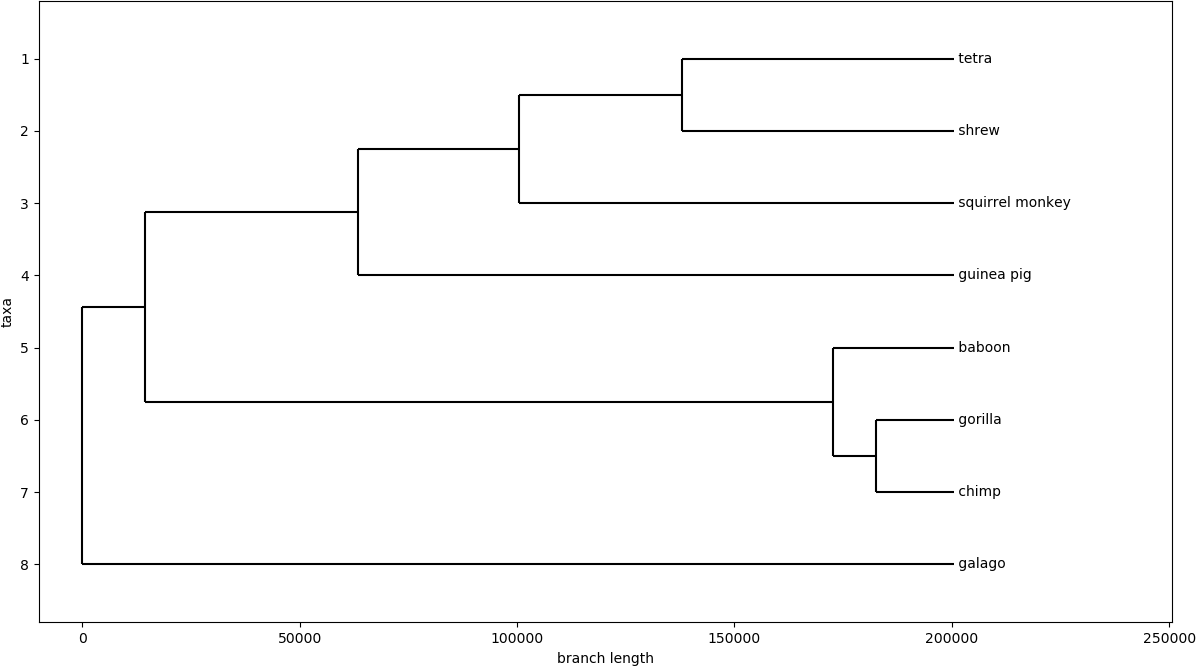
\includegraphics[width=\linewidth]{img/mp_8_taxa_noncoding_2.png}
    \caption{The result of running the exact MP method with branch and bound on 8 elements of the non-coding dataset. Branch lengths have been adjusted to the parsimonious scores of the nodes.}
    \label{fig:mp_noncoding_2}
\end{figure*}

\begin{figure*}
\centering
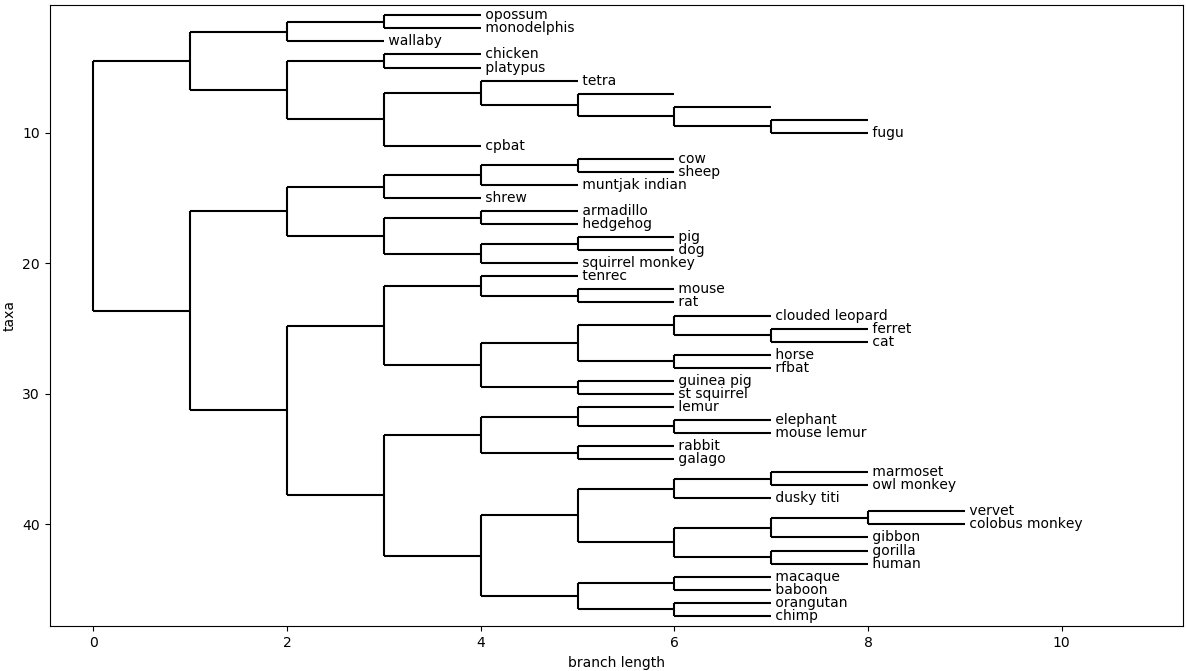
\includegraphics[width=\linewidth]{img/sota_noncoding.png}
\caption{The result of running SOTA on the non-coding dataset.}
\label{fig:sota_noncoding}
\end{figure*}

Neighbor joining performed quite well (Figure \ref{fig:nj_noncoding}); primates are in the same cluster except for \textit{squirrel monkey} and \textit{Glires} (hares, rabbits and rodents) are also together except for \textit{rabbit}, which was instead linked with primates. Cats are still far from dogs, and rats and mice are far from humans, too.

UPGMA (Figure \ref{fig:upgma_noncoding}) produced slightly better results that neighbor joining; the main categories seem stable, although some elements in Laurasiatheria and Glires have been moved around. The tree created with WPGMA (Figure \ref{fig:wpgma_noncoding}) is also remarkable, only some species like \textit{horse} and \textit{vervet}, \textit{dusky titi} and \textit{elephant} deviated from their expected places.

For the sake of simplicity, I decided to make two test runs on 8 taxa instead of one test run on 9 taxa in the case of maximum parsimony. Figure \ref{fig:mp_noncoding_1} is very similar to Figure \ref{fig:mp}; species were chosen to coincide with the ones shown in the non-coding run and as it can be seen there is little or no difference between the two types of sequences in the case of the species selected. Figure \ref{fig:mp_noncoding_2}, although there is no point of comparison from the coding dataset, shows a tree that seems to contain mostly bad taxonomic relationships: according to the tree, primates have diverged early on while \textit{squirrel monkey} is closer to the \textit{guinea pig} than any other primate. This may be due to the lack of information in the non-coding dataset, which contradicts what has been mentioned in correlation with Figure \ref{fig:mp_noncoding_1}; in order to determine if it is really the case, further experimentation with different combinations of species is needed.

Finally, the result of SOTA can be seen in Figure \ref{fig:sota_noncoding}. This is slightly different from the tree shown in Figure \ref{fig:sota}, but the main categories seem to be approximately the same. What is notable is that the algorithm seems to have had a hard time finding the right place for \textit{fugu}. This implies that the parameters are not optimal with respect to rate of convergence. The excess branches may be cut during post-processing.

\section{Conclusion}

Among distance-based methods, WPGMA performed slightly better than NJ and UPGMA on the two datasets. Exact MP with branch and bound could be a good choice as it has produced mostly accurate results, but its running time creates an obstacle in cases with a high number of taxa; heuristic MP with SPR could be a good substitute but there is no guarantee that the sub-optimal result it finds is a sufficiently good one. SOTA is not significantly better than the distance-based methods and its computational complexity is a hindrance to accuracy.

Combining these methods by e.g. starting out from a tree pre-calculated with neighbor joining and then finding better solutions with heuristic MP could result in a possible improvement in performance; such optimization techniques are often used in the field of phylogenetics \cite{Zvelebil2007}. Additionally, it is possible that ML methods give better results than MP methods under special circumstances; finding out which one is better than the other for specific datasets needs extensive experimentation, which I leave for future work.

This study had computational limitations that rendered it impossible to test for a wider range of parameters and produce more results. In most cases, 3 runs is not enough to provide a representative assessment of the methods used, except for the rather simple distance-based algorithms that are deterministic and easy to run. Another thing that was lacking was an objective evaluation metric for the trees. There are some quantitative measures one can take to assess the similarity between different trees (e.g., the Robinson-Foulds metric or the SPR distance metric \cite{Hickey2008}), but there is no standardized way of doing it which makes this task non-trivial. While most of these metrics can be adapted to phylogenetic trees, even rooted ones, comparing them may be out of the scope of this project.

Although the two datasets I used can be considered fairly large, there is certainly demand for more robust techniques in practice. Optimizing and scaling the algorithms I implemented to datasets containing 100+ taxa may also be a good topic for a follow-up project.

The repository is available on \href{https://github.com/Leena01/computational_biology}{GitHub}. Since the project provides a simplified overview of various phylogenetic methods, I hope that it can serve as reference for others who are interested in this field.

\hypersetup{
	urlcolor=black
}
\bibliographystyle{unsrtnat}
\bibliography{report}

\onecolumn
\appendixpage
\appendix
\hypersetup{
	urlcolor=blue
}
\section{Functionality testing}
\label{sec:functionality_testing}

Biopython has its own implementation of the neighbor joining and UPGMA methods. As can be seen in Table \ref{table:distance_biopython} and \ref{table:distance_biopython_2}, these algorithms are a lot faster than mine. This may be due to the fact that their distance matrices were built from scratch instead of relying on Pandas DataFrames.

In addition to comparing the speed, I checked whether my results were similar to theirs. The trees in Figures \ref{fig:nj_coding_bio} and \ref{fig:nj_noncoding_bio} are comparable to the trees in Figures \ref{fig:nj} and \ref{fig:nj_noncoding}, respectively. What is more interesting is that Figures \ref{fig:upgma_coding_bio} and \ref{fig:upgma_noncoding_bio} show UPGMA-based trees that are not ultrametric — that is, the leaves are not equidistant from the root. Moreover, some parts of these trees are different from what I got (shown in Figures \ref{fig:upgma} and \ref{fig:upgma_noncoding}). I checked the \href{https://github.com/biopython/biopython}{source code} of Biopython's \textit{DistanceTreeConstructor} and saw that it does not use weights when calculating new distances (Equation \ref{eq:upgma}). This may be a slightly different version of the original algorithm but seems more like an issue with their implementation. For this reason, the only algorithm I had a benchmark for was neighbor joining; all the other methods were tested with datasets consisting of a small number of sequences (see example in Table \ref{table:test_data}) or unit tests when applicable (e.g., when checking the parsimonious scores produced by Fitch's algorithm).

\begin{minipage}[b]{.475\textwidth}
	\begin{table}[H]
	\caption{Running time of Biopython's implementation of NJ and UPGMA on the coding dataset. 44 taxa are used. The numbers are based on three test runs.}
	\centering
	\begin{tabular}{lll}
		\toprule
		Method & Mean (seconds) & Std. \\
		\midrule
		NJ & 0.0547 & 0.0008 \\
		UPGMA & 0.0493 & 0.0102 \\	
		\bottomrule
	\end{tabular}
	\label{table:distance_biopython}
\end{table}
\end{minipage}%
\hfill
\begin{minipage}[b]{0.475\textwidth}
\begin{table}[H]
	\caption{Running time of Biopython's implementation of NJ and UPGMA on the non-coding dataset. 44 taxa are used. The numbers are based on three test runs.}
	\centering
	\begin{tabular}{lll}
		\toprule
		Method & Mean (seconds) & Std. \\
		\midrule
		NJ & 0.0579 & 0.0029 \\
		UPGMA & 0.0532 & 0.0068 \\	
		\bottomrule
	\end{tabular}
	\label{table:distance_biopython_2}
\end{table}
\end{minipage}

\begin{minipage}[b]{.475\textwidth}
\begin{table}[H]
	\centering
	\begin{tabular}{ll}
		\toprule
		Taxon & Sequence \\
		\midrule
		human & ATGCACGCGGG \\
		chimp & CAGTACGATAG \\
		gorilla & ATGTTCGTCGC \\
		orangutan & GGGGGGGTAAA \\
		\bottomrule
	\end{tabular}
\caption{One of the datasets I created for testing purposes. For a dataset of this size, one can expect that there are multiple optimal solutions.}
\label{table:test_data}
\end{table}

\end{minipage}%
\hfill
\begin{minipage}[b]{0.475\textwidth}
	
\begin{figure}[H]
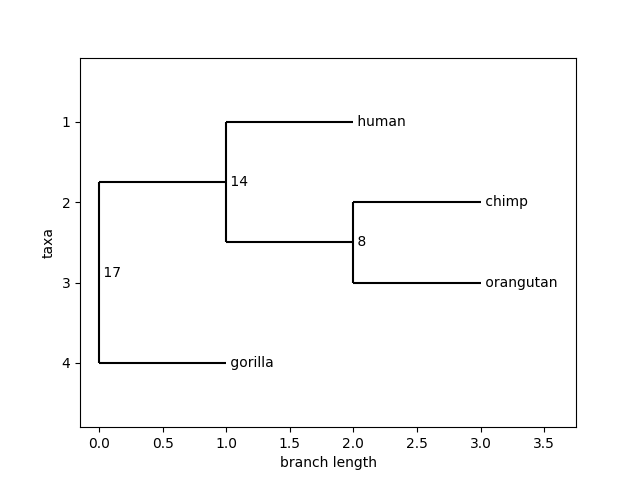
\includegraphics[width=0.98\linewidth]{img/test.png}
\caption{The result of running the exact MP on the test dataset (shown in Table \ref{table:test_data}). Parsimonious scores are shown next to the corresponding inner nodes.}
\label{fig:test}
\end{figure}
\end{minipage}

\begin{figure*}
	\centering
	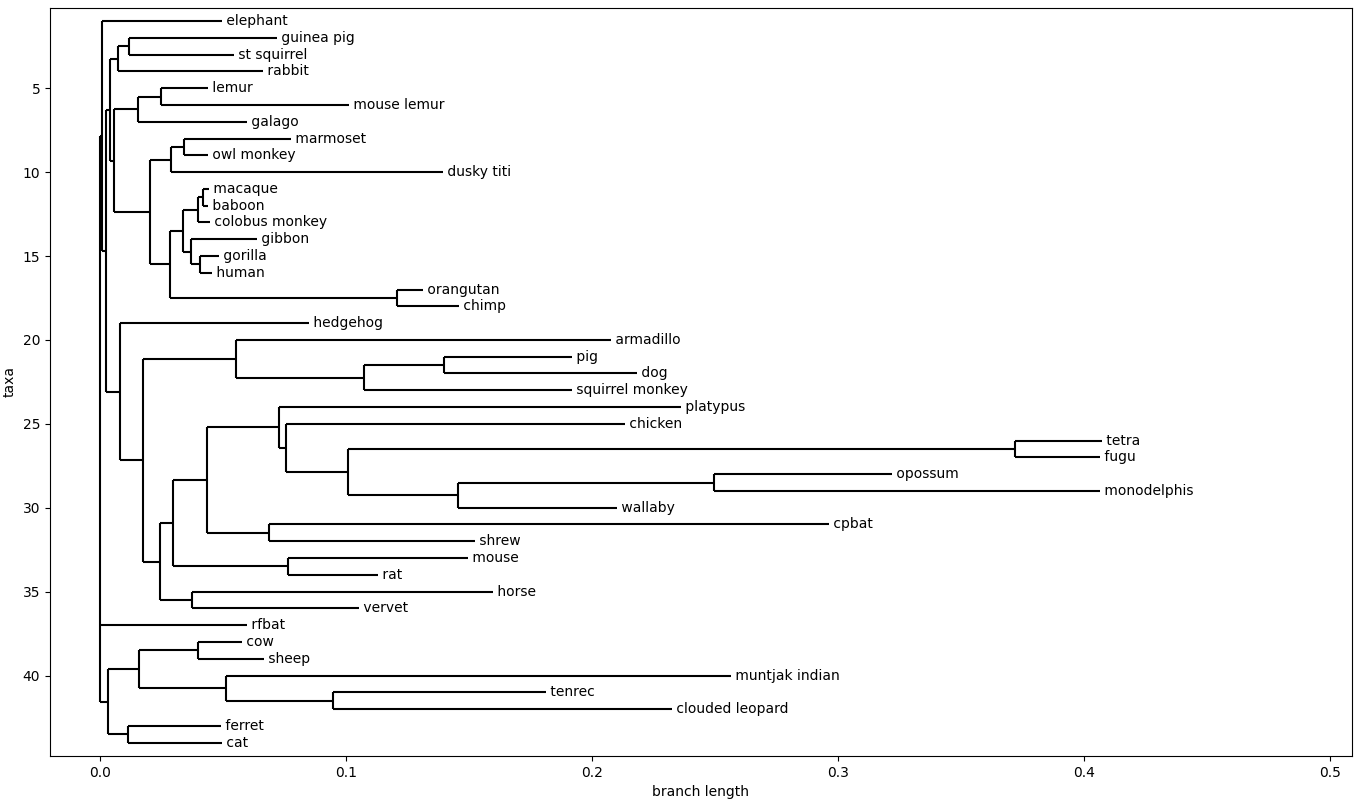
\includegraphics[width=0.95\linewidth]{img/nj_coding_biopython.png}
	\caption{The result of running Biopython's neighbor joining on the coding dataset.}
	\label{fig:nj_coding_bio}
\end{figure*}

\begin{figure*}
\centering
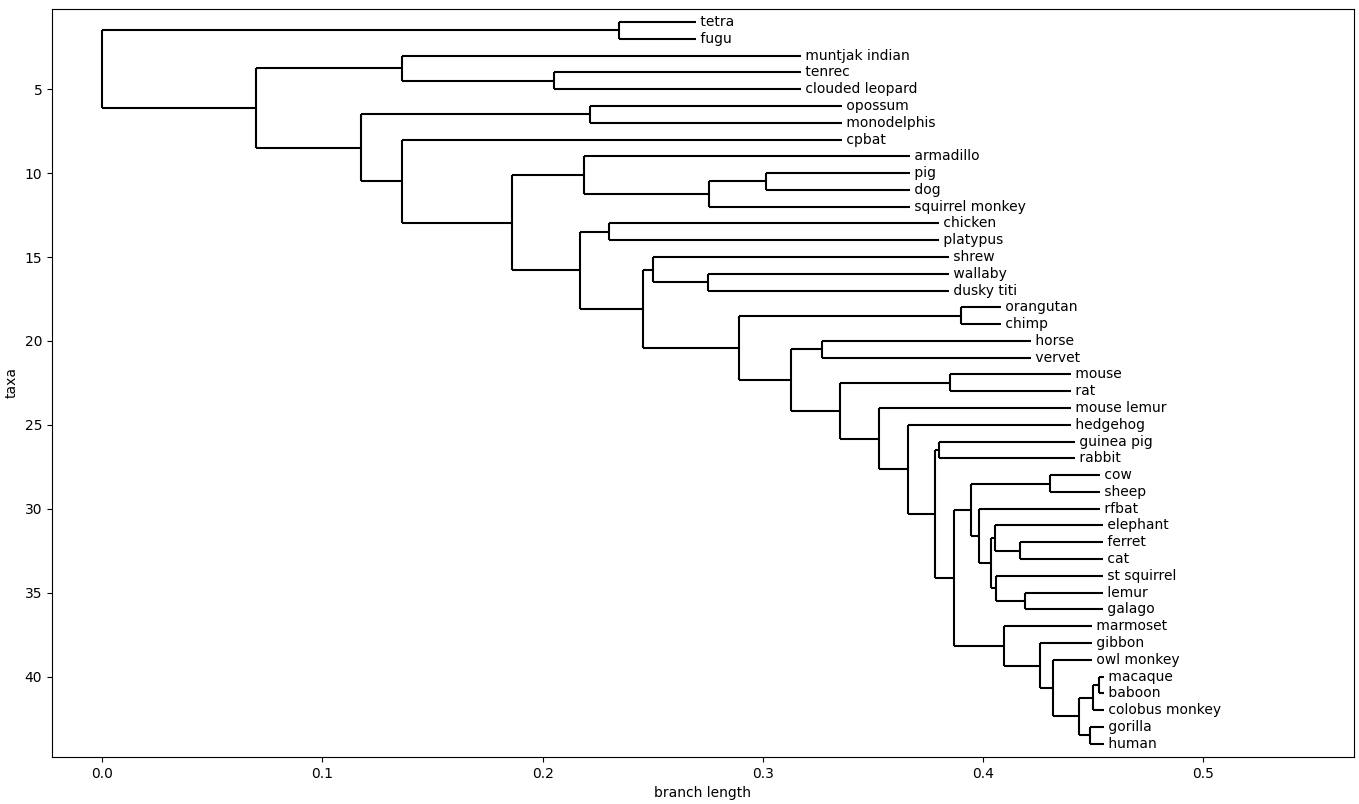
\includegraphics[width=0.95\linewidth]{img/upgma_coding_biopython.png}
\caption{The result of running Biopython's UPGMA on the coding dataset.}
\label{fig:upgma_coding_bio}
\end{figure*}

\begin{figure*}
	\centering
	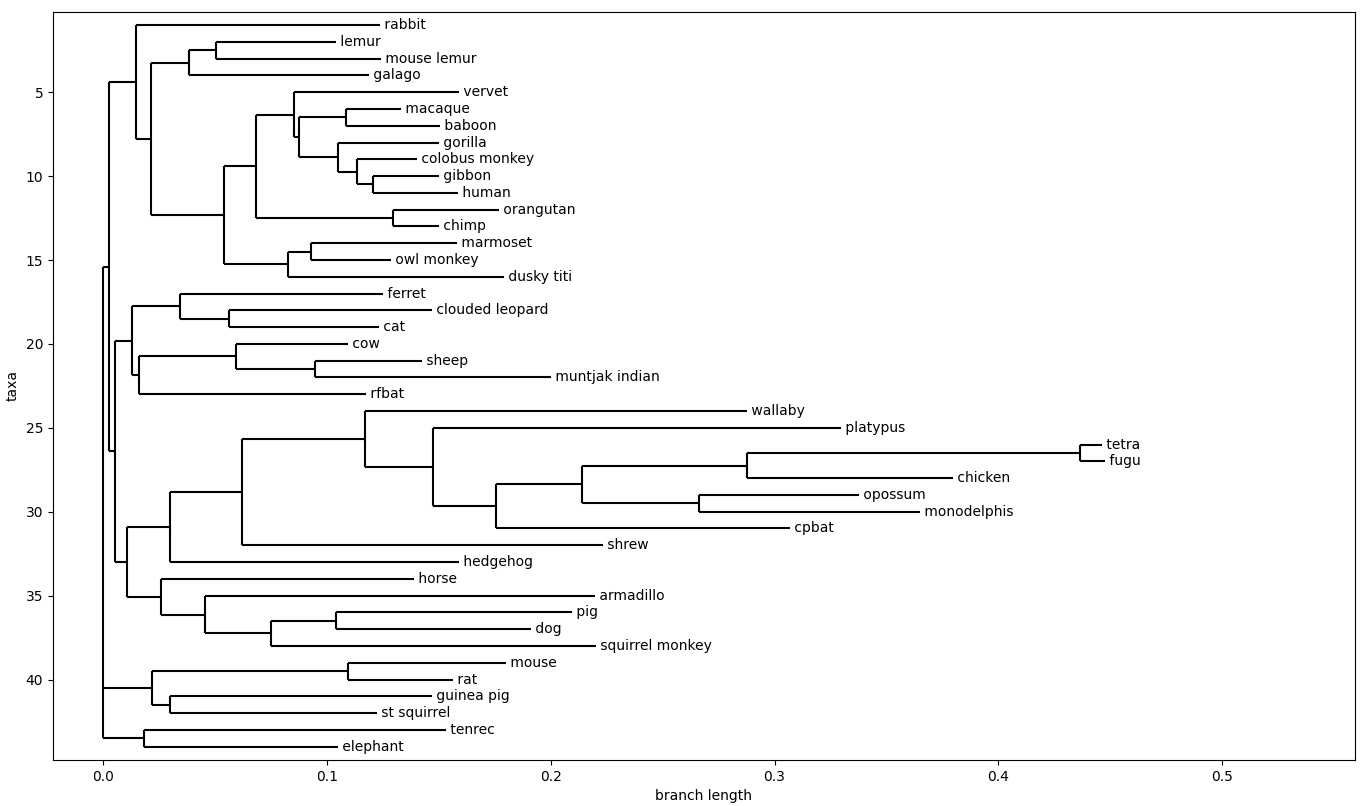
\includegraphics[width=0.95\linewidth]{img/nj_noncoding_biopython.png}
	\caption{The result of running Biopython's neighbor joining on the non-coding dataset.}
	\label{fig:nj_noncoding_bio}
\end{figure*}
\begin{figure*}
	\centering
	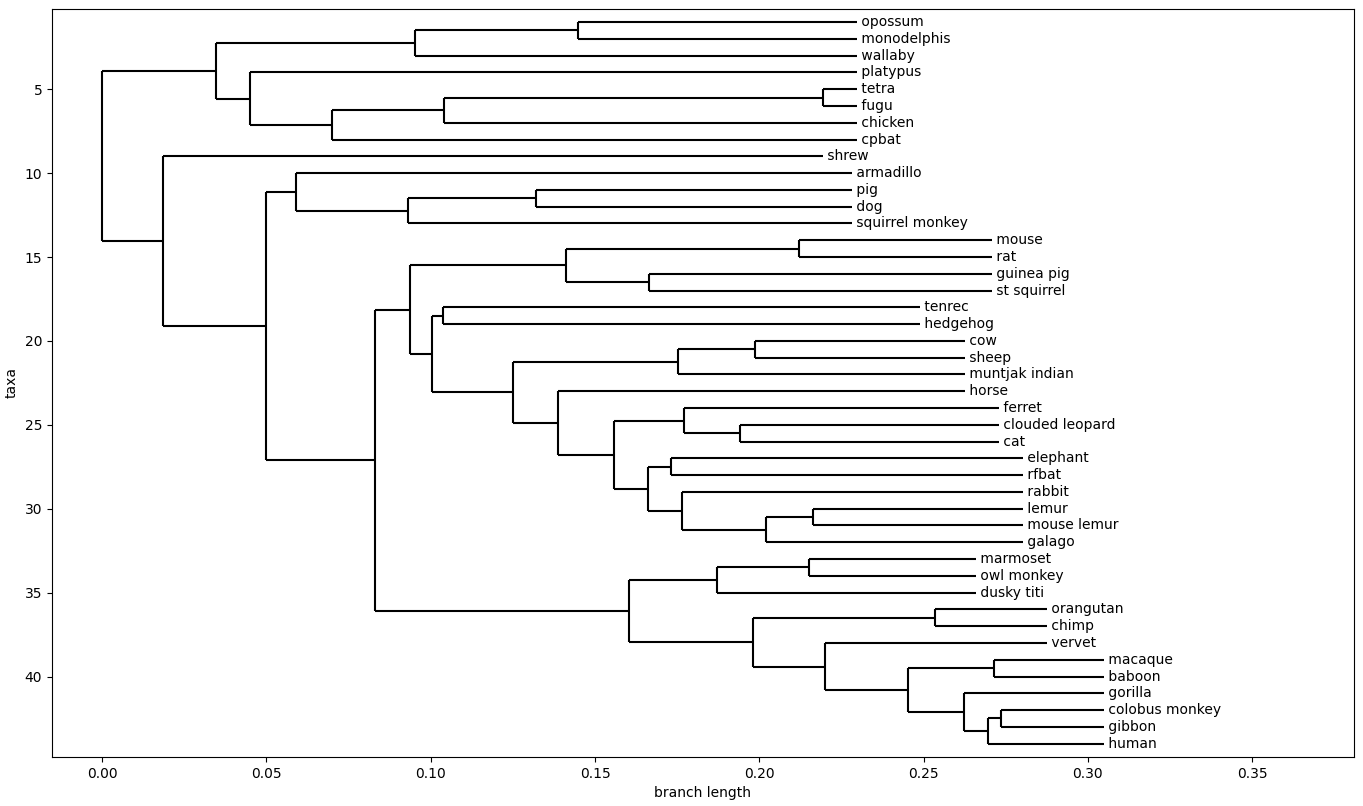
\includegraphics[width=0.95\linewidth]{img/upgma_noncoding_biopython.png}
	\caption{The result of running Biopython's UPGMA on the non-coding dataset.}
	\label{fig:upgma_noncoding_bio}
\end{figure*}

\end{document}
